\documentclass{standalone}
\usepackage{tikz}
\usepackage{tikz-qtree}
\usepackage[makeroom]{cancel}
\usetikzlibrary{fit}


\begin{document} 
	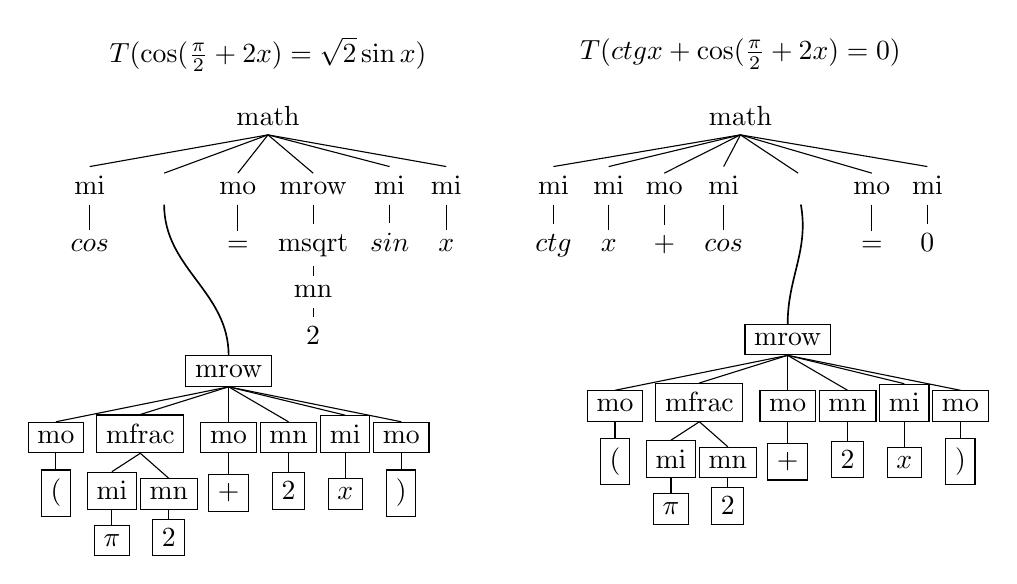
\begin{tikzpicture}[sibling distance=1.2pt]
			\tikzset{level 1/.style={level distance=2.1\baselineskip}}
			\tikzset{level 2/.style={level distance=1.7\baselineskip}}
			\tikzset{level 3+/.style={level distance=1.4\baselineskip}}

		    \node (x) at (0,0.9) {$T(\cos (\frac{\pi}{2} + 2x) = \sqrt{2}\sin x)$};
		    \Tree [.math
		    		[.mi $cos$ ]
		    		[.\node(m2){\phantom{mrow}}; ]
		    		[.mo $=$ ]
		    		[.mrow 
		    			[.msqrt 
		    				[.mn
		    					[.$2$ ]
		    				]
		    			]
		    		]
		    		[.mi $sin$ ]
		    		[.mi $x$ ]
		          ]
	    
		\begin{scope}[xshift=-.5cm, yshift=-3.2cm]
			\tikzset{level 1/.style={level distance=2.0\baselineskip}}
			\tikzset{level 2+/.style={level distance=1.55\baselineskip}}
			\tikzset{level 1+/.style={sibling distance=0.08\baselineskip}}
			\Tree [.\node[draw](m1){mrow}; 
		    			[.\node[draw]{mo}; \node[draw]{$($}; ]
		    			[.\node[draw]{mfrac}; 
		    				[.\node[draw]{mi}; \node[draw]{$\pi$}; ]
		    				[.\node[draw]{mn}; \node[draw]{$2$}; ]
		    			]
		    			[.\node[draw]{mo}; \node[draw]{$+$}; ]
		    			[.\node[draw]{mn}; \node[draw]{$2$}; ]
		    			[.\node[draw]{mi}; \node[draw]{$x$}; ]
		    			[.\node[draw]{mo}; \node[draw]{$)$}; ]
		    	  ]
			\draw[semithick,-] (m1) to [out=90, in=270] (m2);
			%\node (edge) at (-2.5,-2) {\phantom{X}}; 
			%\node (ph1) at (-2.3,-2) {\phantom{X}}; 
			%\node (ph2) at (2.3,0) {\phantom{X}}; 
			%\node[draw,dashdotted,fit=(ph1)(ph2)]{};
		\end{scope}

		\begin{scope}[xshift=6cm]
			\tikzset{level 1/.style={level distance=2.1\baselineskip}}
			\tikzset{level 2/.style={level distance=1.7\baselineskip}}
			\tikzset{level 3+/.style={level distance=1.4\baselineskip}}

		    \node (x) at (0,0.9) {$T(ctg x + \cos (\frac{\pi}{2} + 2x) = 0)$};
		    \Tree [.math
		    		[.mi $ctg$ ]
		    		[.mi $x$ ]
		    		[.mo $+$ ]
		    		[.mi $cos$ ]
		    		[.\node(m2){\phantom{mrow}}; ]
		    		[.mo $=$ ]
		    		[.mi $0$ ]
		          ]
		\end{scope}


		\begin{scope}[xshift=6.6cm, yshift=-2.8cm]
			\tikzset{level 1/.style={level distance=2.0\baselineskip}}
			\tikzset{level 2+/.style={level distance=1.55\baselineskip}}
			\tikzset{level 1+/.style={sibling distance=0.08\baselineskip}}
			\Tree [.\node[draw](m1){mrow}; 
		    			[.\node[draw]{mo}; \node[draw]{$($}; ]
		    			[.\node[draw]{mfrac}; 
		    				[.\node[draw]{mi}; \node[draw]{$\pi$}; ]
		    				[.\node[draw]{mn}; \node[draw]{$2$}; ]
		    			]
		    			[.\node[draw]{mo}; \node[draw]{$+$}; ]
		    			[.\node[draw]{mn}; \node[draw]{$2$}; ]
		    			[.\node[draw]{mi}; \node[draw]{$x$}; ]
		    			[.\node[draw]{mo}; \node[draw]{$)$}; ]
		    	  ]
			\draw[semithick,-] (m1) to [out=90, in=280] (m2);
		\end{scope}


	\end{tikzpicture}
\end{document} 